\documentclass[margin=3.15mm]{standalone}
\usepackage{tikz}

\begin{document}

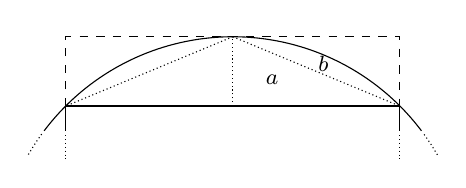
\begin{tikzpicture}

    % Define radius of the circle
    \def\radius{3}
    
    % Draw the arc of the circle from 45º to 135º
    \draw (37:\radius) arc[start angle=37, end angle=143, radius=\radius];
    \draw [densely dotted] (30:\radius) arc[start angle=30, end angle=36, radius=\radius, densely dotted];
    \draw [densely dotted] (144:\radius) arc[start angle=144, end angle=150, radius=\radius, densely dotted];
    
    % Draw the inscribed square
    % \draw (-2.12, 2.12) -- (2.12, 2.12) -- (2.12, -2.12) -- (-2.12, -2.12) -- cycle;
    % \draw (-2.12, 2.12) -- (2.12, 2.12);
    \draw (-2.12, 2.12) -- (-2.12, 1.8);
    \draw (2.12, 2.12) -- (2.12, 1.8);
    \draw [densely dotted] (-2.12, 1.75) -- (-2.12, 1.45);
    \draw [densely dotted] (2.12, 1.75) -- (2.12, 1.45);
    \draw [dashed] (-2.12, 2.12) -- (-2.12, 3) -- (2.12, 3) -- (2.12, 2.12) -- (-2.12, 2.12);
    
    % Draw a dashed rectangle connecting the top of the circle (at 90º) and the square's corners
    % Top of the circle at 90º
    \draw[densely dotted] (0, \radius) -- (-2.12, 2.12);  % Left side of the rectangle
    \draw[densely dotted] (0, \radius) -- (2.12, 2.12);   % Right side of the rectangle
    \draw (-2.12, 2.12) -- (2.12, 2.12);  % Bottom side of the rectangle
    \draw [densely dotted] (0, 2.12) -- (0, 3);  % Bottom side of the rectangle

    \node at (0.5, 2.45) {\footnotesize $a$};
    \node at (1.15, 2.65) {\footnotesize $b$};
    
    % Label points
    % \node at (0, \radius + 0.3) {90º (top of the arc)};
    % \node at (-2.6, 2.12) {45º};
    % \node at (2.6, 2.12) {135º};

\end{tikzpicture}

\end{document}
